\documentclass{article}[12pt]

\usepackage[utf8]{inputenc}
\usepackage{amsmath}
\usepackage{graphicx}
\usepackage{subcaption}
\usepackage{float}
\usepackage[a4paper, margin=1in]{geometry}
\usepackage{hyperref}

\graphicspath{./images/}

\title{Création d’une plateforme pour l’analyse du signal posturographique \\
\textbf{Deuxième semaine}}
\author{Inès PINGAULT, Anaëlle MAZOUNI, Hippolyte DEPARIS \\
Lille }

\date{\today}

\begin{document}
\maketitle

\newpage
\tableofcontents

\newpage
\section{Introduction}

La posturographie, aussi appelée posturologie, est une technique employée pour évaluer, 
mesurer et contrôler la posture en position debout. Pour maintenir un équilibre vertical, 
le corps humain ajuste en permanence sa posture par rapport à son environnement en fonction de 
certains signaux qu'il reçoit. Ces signaux sont captés par les yeux, la colonne vertébrale, 
l’oreille interne ou encore les pieds. Le cerveau les analyse et envoie des instructions au 
corps dans le but de modifier sa posture en temps réel aux différents éléments perçus. Si ces 
signaux, importants pour le maintien de l'équilibre ne sont pas ou mal perçus, ou mal analysés,
la posture ne sera pas correctement adaptée, et des troubles tels que des déséquilibres, des 
vertiges ou encore des problèmes musculosquelettiques pouvant aller jusqu'à des douleurs 
chroniques dans certaines régions de l’organisme pourraient apparaître. Il est donc important 
pour les posturologues de mettre aujourd’hui l’accent sur l'étude du rôle des yeux, des pieds 
ainsi que les occlusions dentaires dans les problèmes liés à la posture. Cette discipline étudie
la position de l’homme dans l’espace (son équilibre, sa stature, son aplomb, sa stabilité...)
grâce à des appareils de mesure spécialisés. Elle prend en compte la capacité de rester en 
équilibre sur ses pieds ainsi que la symétrie du corps ou la perception visuelle de 
l'horizontalité. Ces études sont possibles aussi bien dans des situations statiques que 
dynamiques. La posturographie dynamique informatisée (non étudiée dans ce rapport) est une 
technique d’évaluation clinique non invasive permettant de quantifier les mécanismes
d’adaptation du système nerveux central lorsque le corps est en mouvement (Figure 1).  
La posturographie statique évalue quant à elle la posture d’un patient en équilibre
orthostatique (position érigée immobile, fondamentale de l'espèce humaine). Cette évaluation
se fait en positionnant debout, le patient sur une plateforme équipée de nombreux capteurs 
de pression. L’enregistrement des oscillations du centre de pression des pieds permettent 
de retracer l'évolution du centre de gravité (ou centre de masse) du patient. Lors de ces 
évaluations, on étudie aussi la réponse posturale du patient à certaines perturbations 
(Figure 2).


\begin{figure}[ht]
    \centering
    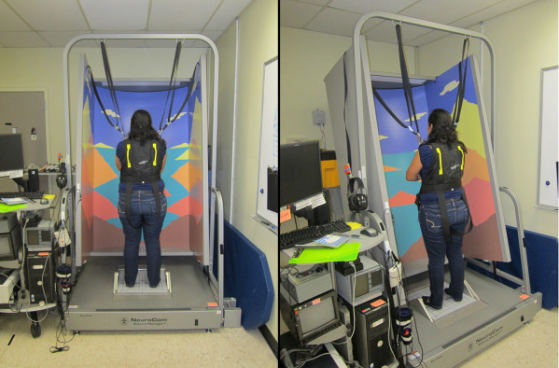
\includegraphics[width=0.5\textwidth]{images/introduction/dynamique.png}
    \caption{Machine d’analyse de la posturographie dynamique }
    \label{fig:posturographie-dynamique}
\end{figure}

\begin{figure}[ht]
    \centering
    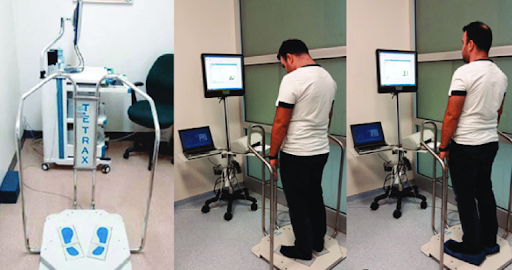
\includegraphics[width=0.5\textwidth]{images/introduction/statique.png}
    \caption{Machine d’analyse de la posturographie statique }
    \label{fig:posturographie-statique}
\end{figure}



\newpage
\section{Signal analysé en posturographie statique}

\subsection{Pression plantaire}

Les pressions plantaires mesurent la répartition des forces sous les pieds au niveau des zones d’appui.
Ces pressions sont capturées par des capteurs disposés sur une surface ou intégrées dans des semelles.
Ces mesures permettent d’identifier les points de pression maximale et minimale, fournissant des données sur la statique et la dynamique du pied.
Les centres de pression sont calculés à partir des variations de pression.
Ils reflètent les ajustements dynamiques de la posture en réponse aux déséquilibres.
Les mesures de ces signaux nous permettent de cartographier les zones d'appui et de visualiser les charges appliquées sur les pieds.
On peut alors identifier les zones à risque de pathologie (comme l’hallux valgus ou la fasciite plantaire).
L'évaluation des déséquilibres ou anomalies dans la distribution des forces est alors possible.
Les études sont appliquées en podologie et orthopédie, pour détecter les troubles plantaires ou les anomalies posturales.
Elles sont aussi utilisées pour suivre les progrès post-blessures ou post-chirurgie de patients.
Enfin, on peut aussi les mener dans le but d’optimiser les performances athlétiques en analysant les impacts au sol.

\subsection{Méthode d'enregistrement}

Les plateformes stabilométriques mettent l’accent sur l'étude des mouvements posturaux en évaluant les forces verticales et les déplacements dans les plans horizontal et vertical.
Ces plateformes disposent fréquemment d’instruments additionnels, comme des surfaces instables ou des systèmes de visualisation interactifs pour perturber l'équilibre et examiner les réactions compensatoires du patient.
Ces dispositifs sont utilisés pour évaluer la stabilité posturale en position debout, notamment chez des patients atteints de troubles neurologiques ou vestibulaires.
Ils sont également utilisés pour détecter les déficiences proprioceptives et pour la rééducation.
En gériatrie, ils permettent d'évaluer les risques de chute, et en sport, ils servent à optimiser les stratégies d' équilibre.\\

\textbf{Exemples :}
\begin{itemize}
  \item Stabilo Stabilometric Platform
  \item Plateforme Satel
\end{itemize}

\begin{figure}[H]
 \centering
  \begin{subfigure}[b]{0.45\textwidth}
    \centering
    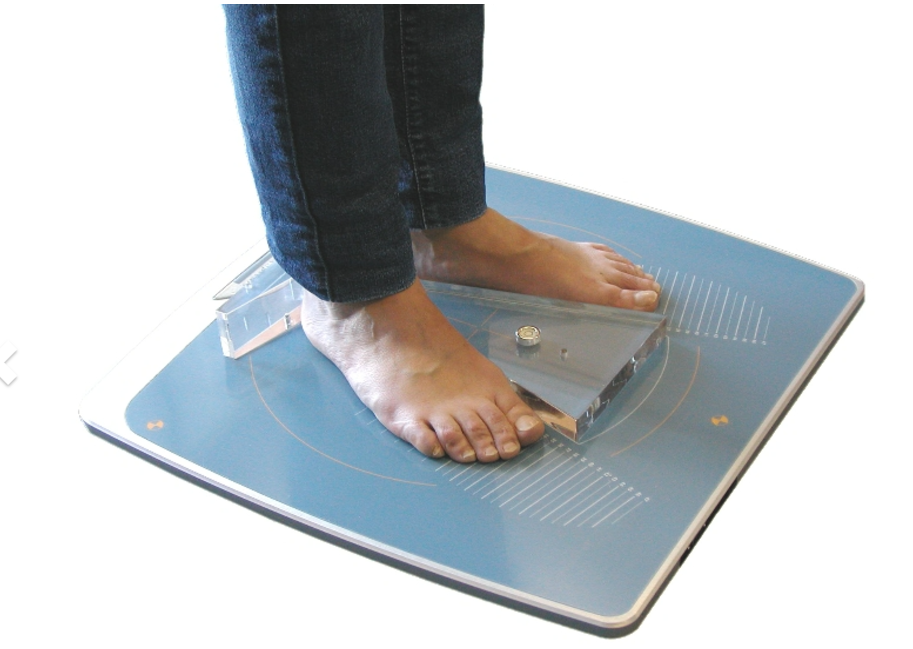
\includegraphics[height=5cm]{images/pression_plantaire/plateforme-stabilometrique.png}
    \caption{Plateforme stabilométrique}\label{fig:plateforme_stabilometrique}
  \end{subfigure}
  \begin{subfigure}[b]{0.45\textwidth}
   \centering
    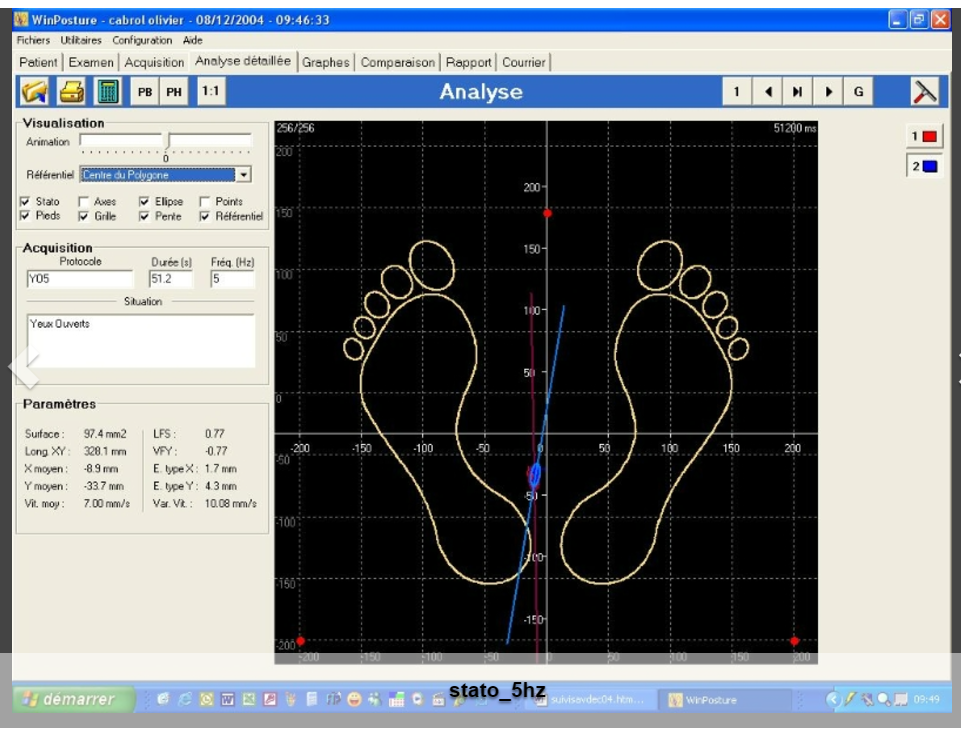
\includegraphics[height=5cm]{images/pression_plantaire/winposture.png}
    \caption{Logiciel de visualisation Winposture}\label{fig:winposture}
  \end{subfigure} \\
  \begin{subfigure}[b]{0.45\textwidth}
    \hspace{-1.5cm}
    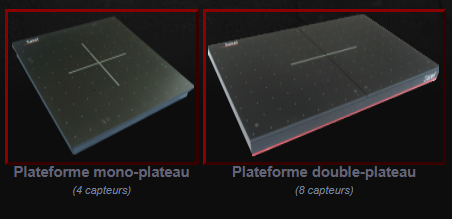
\includegraphics[height=5cm]{images/pression_plantaire/satel.png}
    \caption{Plateforme stabilométrique Satel}\label{fig:satel}
  \end{subfigure}
  % \caption{Ill}\label{fig:exemple_plateforme_force}
\end{figure}

\begin{figure}[ht]
  \centering
  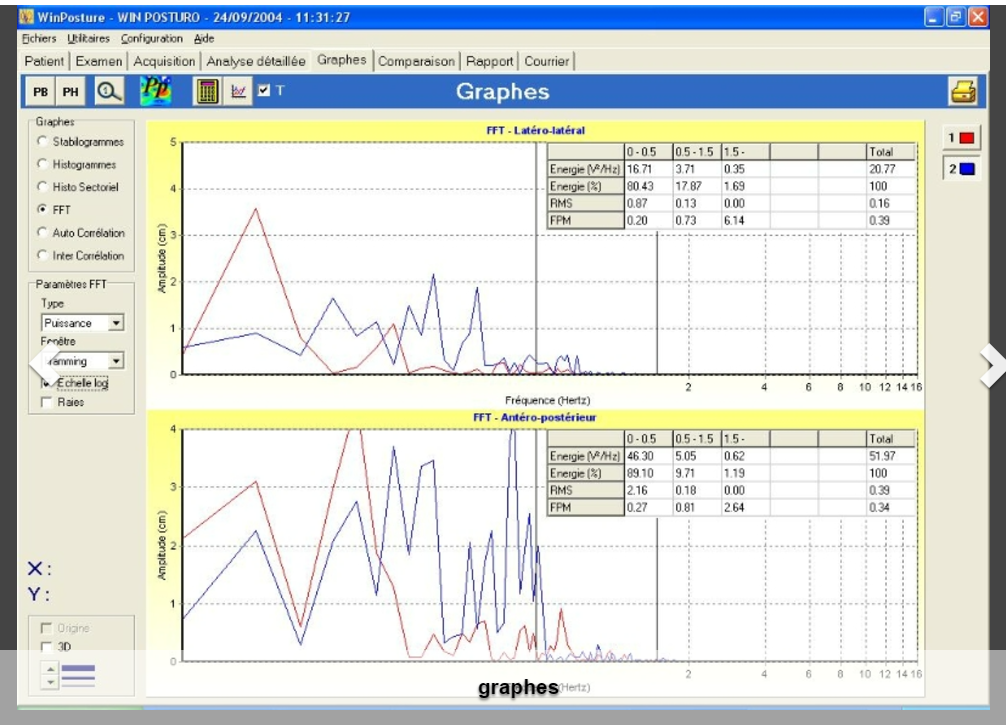
\includegraphics[height=10cm]{images/pression_plantaire/winposture2.png}
  \caption{Logiciel Winposture}\label{fig:winposture2}
\end{figure}


\newpage
\section{Analyse de marché}

\subsection{Win-posturo}


WIN-POSTURE NV Software est une plateforme d'analyse en posturographie statique. 
Elle se distingue par sa convivialité et son ergonomie, facilitant son utilisation. 
Il offre la possibilité de créer et de gérer des protocoles d'acquisition tout en permettant de paramétrer des normes conformes aux recommandations de l'AFP85 (SOFPEL). 
Ce logiciel intègre des fonctionnalités avancées telles que l'analyse fractale et l'analyse par ondelette. 
Il permet également de comparer les résultats des examens pour chaque patient, avec des données facilement exportables vers Excel. 
Les rapports et bilans générés sont entièrement personnalisables, et le logiciel propose des outils intégrés pour la création de courriers et le publipostage.


WIN-POSTURE NV Software une nouvelle plateforme d’analyse de stabilographie statique qui a comme fonctionnalités : 
\begin{itemize}
    \item \textbf Convivialité et ergonomie incomparables.
    \item \textbf Création et gestion des protocoles d’acquisition
    \item \textbf Paramétrage des normes et référentiels 
    \item \textbf Production de la totalité des données stabilométriques normalisées APE 85
    \item \textbf Nouvelles fonctionnalités issues de l’actualité scientifique (option : ondelettes, analyses fractales et de diffusion…) 
    \item \textbf Possibilité de comparaison des examens 
    \item \textbf Multiples Visualisations du signal stabilométrique 
    \item \textbf Edition de rapports et bilans personnalisables  
    \item \textbf Exportation directe des données stabilométriques vers Excel 
    \item \textbf Editeur de courrier 
    \item \textbf publipostage
\end{itemize}

\begin{figure}[H]
    \centering
    \begin{subfigure}[b]{0.45\textwidth}
      \centering
      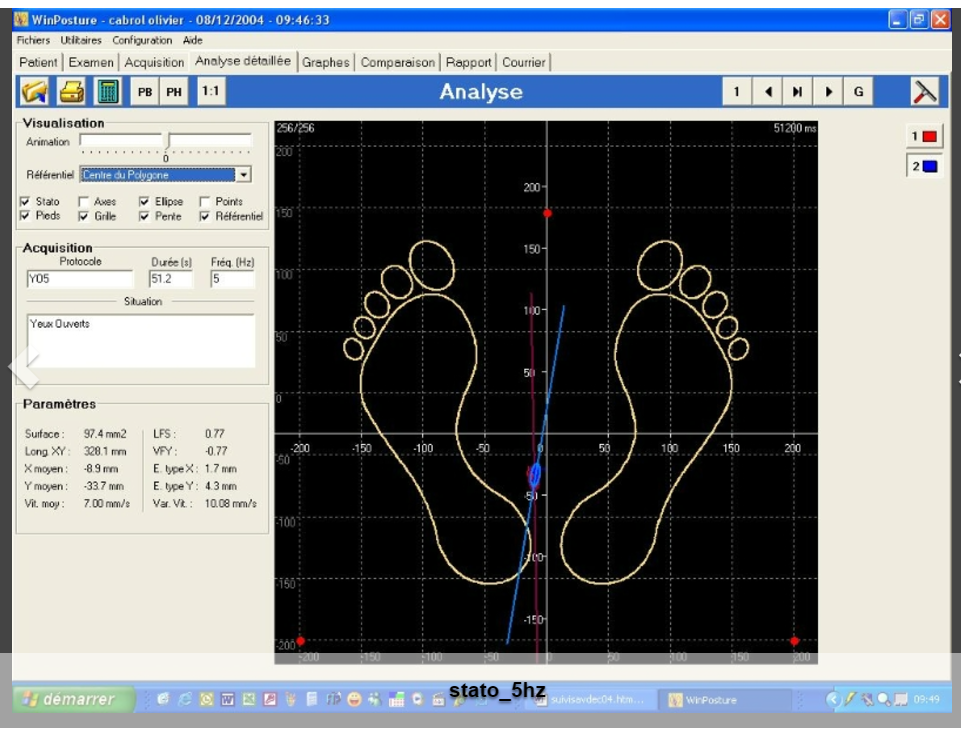
\includegraphics[height=5cm]{images/pression_plantaire/winposture.png}
      \caption{Logiciel Winposture}\label{fig:winposture}
    \end{subfigure}
    \begin{subfigure}[b]{0.5\textwidth}
        \centering
        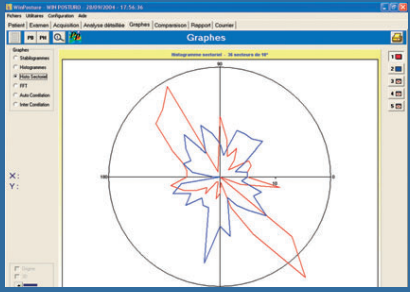
\includegraphics[height=5cm]{images/analyse_marche/winposture_ellipse.png}
        \caption{Visualisation de l'ellipse de confiance}\label{fig:winposture_ellipse_de_confiance}
    \end{subfigure}
    \begin{subfigure}[b]{0.5\textwidth}
        \centering
        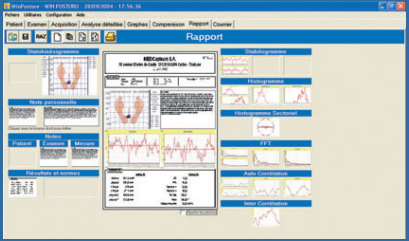
\includegraphics[height=5cm]{images/analyse_marche/winposture_rapport.png}
        \caption{Rapport du logiciel sur un cas patient}\label{fig:winposture_rapport}
    \end{subfigure}
    \begin{subfigure}[b]{0.5\textwidth}
        \centering
        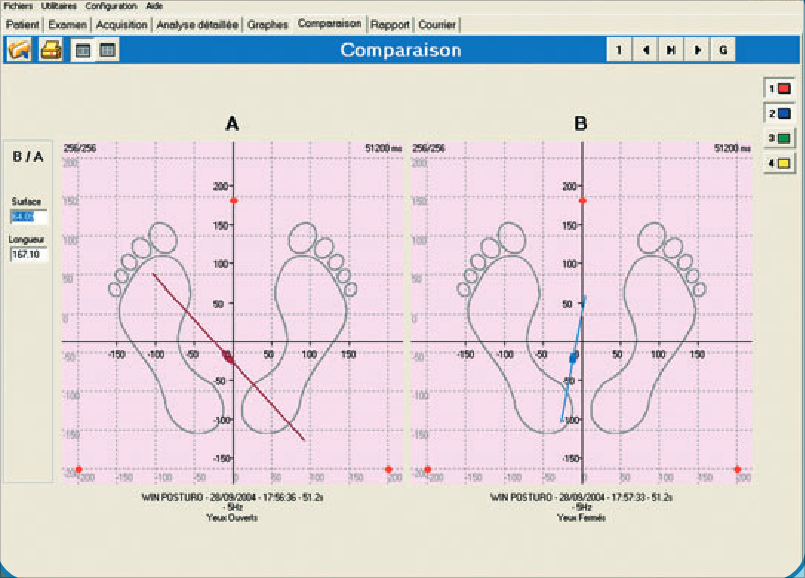
\includegraphics[height=5cm]{images/analyse_marche/comparaison_yo_yf.png}
        \caption{Comparaison de l'équilibre orthostatique yeux ouverts/fermés}\label{fig:winposture_comparaison_yo_yf}
    \end{subfigure}
\end{figure}

\subsection{Fusyo}

Fusyo combine analyses stabilométriques et baropodométriques pour une évaluation complète de \\ l'équilibre et des pressions plantaires. 
Cette plateforme d'analyse se distingue par ses visualisations avancées, notamment en thermographie, 3D et isopression. 
Il inclut des indicateurs tels que le Foot Posture Index, offrant une précision précieuse pour des analyses cliniques approfondies. 
Il permet de créer et gérer des protocoles d'acquisition tout en fournissant des données stabilométriques normalisées selon l'APE 85. 
Les résultats sont personnalisables et peuvent être facilement comparés entre les examens.

Fusyo combine analyses stabilométriques et baropodométriques pour une évaluation complète 
de l’équilibre et des pressions plantaires. 
Cette plateforme d’analyse a comme fonctionnalités:

\begin{itemize}

    \item \textbf Analyse statique 
    \item \textbf Cartographie statique avec calcul par zone 
    \item \textbf Multitude de visualisations (thermographique, isopression, pourcentage, 3D...)  
    \item \textbf Impression à l’échelle 1/1 
    \item \textbf Comparaison d’examens
    \item \textbf Rapport personnalisable : insertion de photos, ajout de commentaires, création de modèles types, impression à la file 
     \item \textbf Possibilité de lier des documents électroniques à un examen 
     \item \textbf Exportation au format PDF 
    \item \textbf Gestion d’un agenda multi-praticiens
    \item \textbf Convivialité et ergonomie incomparables 
    \item \textbf Création et gestion des protocoles d’acquisition 
    \item \textbf Paramétrage des normes et référentiels 
    \item \textbf Production de la totalité des données stabilométriques normalisées APE 85 
    \item \textbf Nouvelles fonctionnalités issues de l’actualité scientifique (option : ondelettes, analyses fractales et de diffusion…) 
    \item \textbf Possibilité de comparaison des examens 
    \item \textbf Multiples visualisations du signal stabilométrique 
    \item \textbf Edition de rapports et bilans personnalisables 
    \item \textbf Exportation directe des données stabilométriques vers Excel 
    \item \textbf Editeur de courrier 
    \item \textbf Publipostage
    
\end{itemize}

\begin{figure}[H]
    \centering
    \begin{subfigure}[b]{0.45\textwidth}
        \centering
      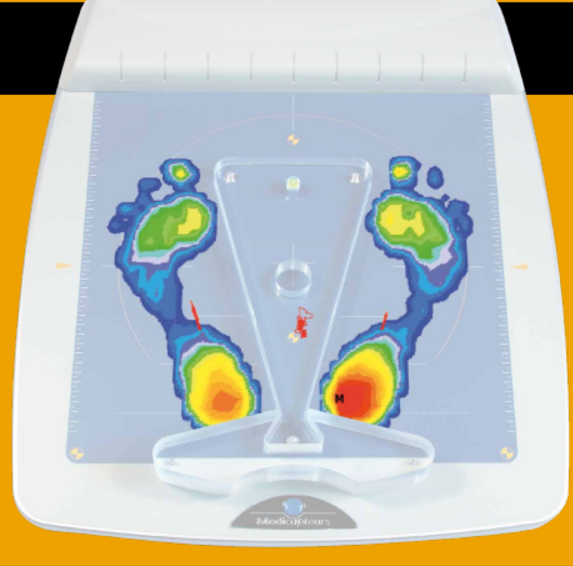
\includegraphics[height=5cm]{images/analyse_marche/Fusyo_1.png}
      \caption{Plateforme d'analyse Fusyo}\label{fig:Fusyo_1}
    \end{subfigure}\\
    \begin{subfigure}[b]{0.45\textwidth}
        \hspace{-4.5cm}
        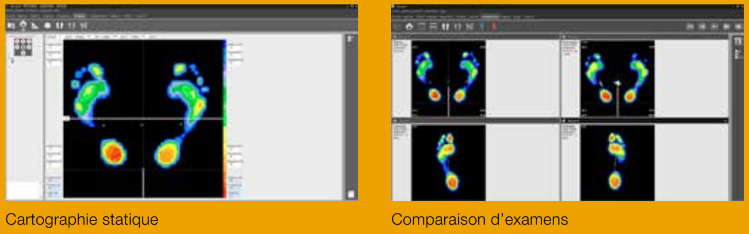
\includegraphics[height=5cm]{images/analyse_marche/Fusyo_2.png}
        \caption{Outils de comparaison des cartographies statiques}\label{fig:Fusyo_2}
    \end{subfigure}\\
    \begin{subfigure}[b]{0.45\textwidth}
        \hspace{-5cm}
        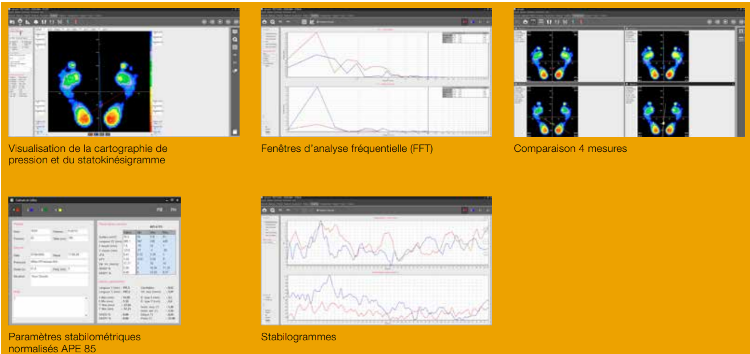
\includegraphics[height=8cm]{images/analyse_marche/Fusyo_4.png}
        \caption{Outils de visualisations des données stabilométriques}\label{fig:Fusyo_4}
    \end{subfigure}
\end{figure}

\subsection{FOOTWORK PRO}

FootWork Pro est conçu pour les analyses statiques et dynamiques. 
Il inclut des fonctionnalités avancées telles que centre des pressions, 
pression maxi de chaque pied, répartition avant et arrière, droite et gauche. 
Projection du centre de gravité, zone d’études et film de la statique.  
Possibilité de paramétrer la durée, la fréquence et le pourcentage des points.
Il est compatible avec les ordinateurs Windows, cette plateforme d’analyse est simple à intégrer 
dans des environnements de travail classiques.
Il permet l'édition des comptes rendus et permet la possibilité d’envoi par mail 
des analyses avec création des fichiers patients.

FootWork Pro est conçu pour les analyses statiques. 
Cette plateforme d’analyse a comme fonctionnalités:

\begin{itemize}
    \item \textbf Fichier patients
    \item \textbf Analyse statique : centre des pressions, pression maxi de chaque pied, répartition avant et arrière, droite et gauche. Projection du centre de gravité, zone d’études et film de la statique.
    \item \textbf Stabilométrie : ellipses et dimensions des centres de poussée. Oscillation et pourcentage en surface et en temps : plan frontal, sagittal. Possibilité de paramétrer la durée, la fréquence et le pourcentage des points. Analyse unipodale.
    \item \textbf Analyse dynamique : pas multiples avec reconnaissance automatique pied droit / pied gauche. Pressions moyennes et maxi, durée d’appui et intégrale pression / temps. Zones d’études : précise les zones de travail du pied. Automatiques, intelligentes, manuelles et médio-latérale. Analyse des 3 temps du pas avec superposition d'une référence. Vidéo 3D.
    \item \textbf Compatible PC Windows uniquement.
    \item \textbf Editions des comptes rendus et possibilité d’envoi par mail des analyses.
    \item \textbf Inclus 3 ans de contrat d’assistance et de mise à jour
\end{itemize}

\begin{figure}[H]
    \centering
    \begin{subfigure}[b]{0.45\textwidth}
      \centering
        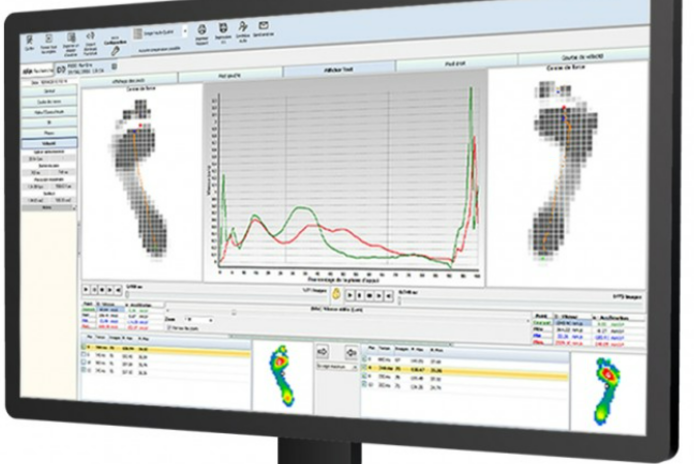
\includegraphics[height=5cm]{images/analyse_marche/Footwork_pro.png}
        \caption{Outil de visualisation des données posturographiques FootWork}\label{fig:Footwork_pro}
    \end{subfigure}
    \begin{subfigure}[b]{0.5\textwidth}
        \centering
        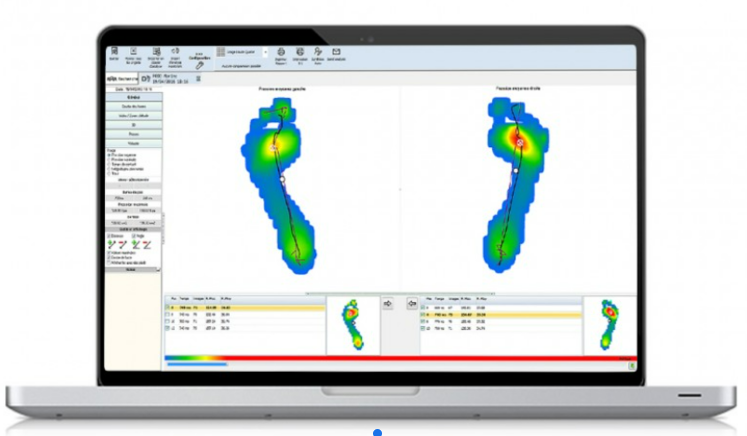
\includegraphics[height=5cm]{images/analyse_marche/Footwork_pro_1.png}
        \caption{Outil de visualisation 3D des centre de pression Footwork}\label{fig:Footwork_pro1}
    \end{subfigure}
    \begin{subfigure}[b]{0.5\textwidth}
        \centering  
        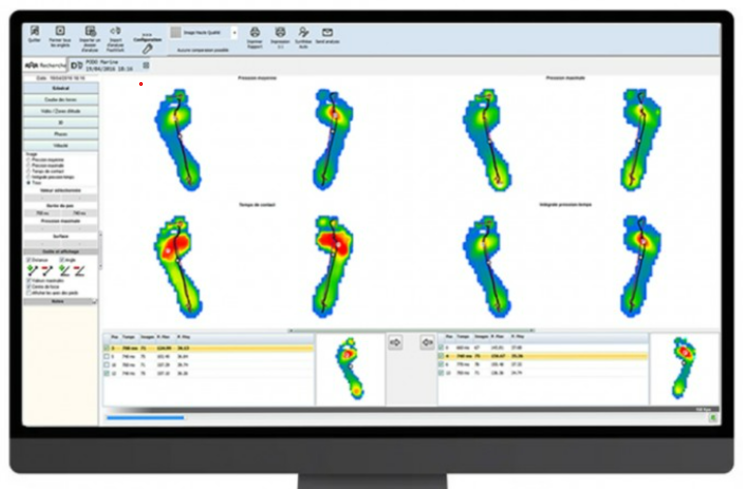
\includegraphics[height=5cm]{images/analyse_marche/Footwork_pro_2.png}
        \caption{Outil de comparaison des models 3D Footwork}\label{fig:Footwork_pro2}
    \end{subfigure}
\end{figure}


\subsection{Win-pod}

WinPod est une solution intuitive destinée aux analyses posturales simples 
et qualitatives. Il permet de personnaliser les rapports en y ajoutant photos, 
commentaires et modèles prédéfinis. En temps réel, il génère des cartographies et
 suit l’évolution des centres de pression. Cependant, WinPod est limité en termes 
 d’analyses avancées et convient mieux aux besoins cliniques de base ou aux bilans 
 qualitatifs qu’aux études approfondies.

 WinPod est une solution intuitive destinée aux analyses posturales 
 simples et qualitatives. Cette plateforme d’analyse a comme fonctionnalités:

\begin{itemize}
    \item \textbf Cartographie statique avec calcul par zone
    \item \textbf Multitude de visualisations (thermographique, isopression,3D…)
    \item \textbf Analyse numérique et graphique des paramètres de stabilométrie
    \item \textbf Evolution des cartographies et des centres de pression
    \item \textbf Quotient de Romberg
    \item \textbf Visualisation temps réel
    \item \textbf Archivage de tout type de documents électronique à la fiche d’examen clinique
    \item \textbf Rapport personnalisable : insertion de photos, ajout, de commentaires
    \item \textbf Exportation au format PDF
    \item \textbf Intégration du foot posture index FPI (Normalisation internationale du pied)
    \item \textbf Calcul du CPEI (Centre of Pressure Foot Index)
    \item \textbf Impression à l'échelle 1/1
    \item \textbf Comparaison d’examens
    \item \textbf File d’impression

\end{itemize}

 \begin{figure}[H]
    \centering
    \begin{subfigure}[b]{0.45\textwidth}
      \centering
        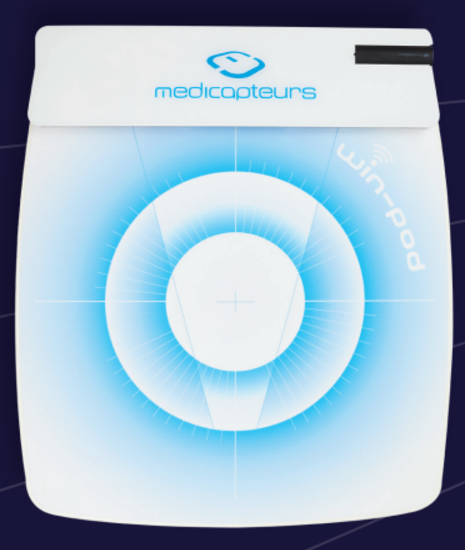
\includegraphics[height=5cm]{images/analyse_marche/WinPod.png}
        \caption{Plateforme stabilométriques Win-pod}\label{fig:WinPod}
    \end{subfigure}
    \begin{subfigure}[b]{0.5\textwidth}
        \centering
        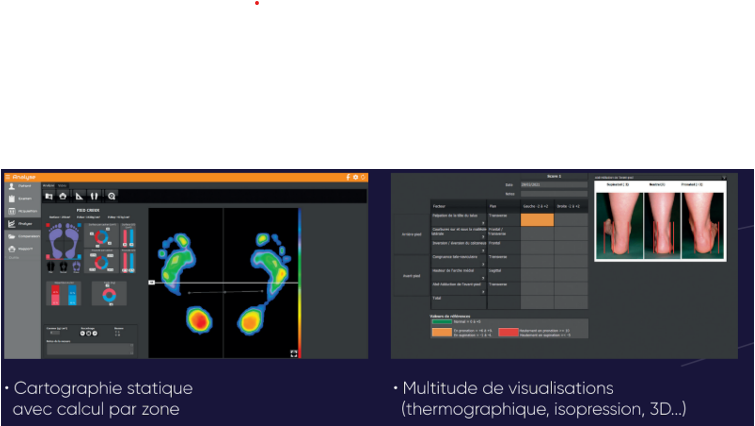
\includegraphics[height=5cm]{images/analyse_marche/WinPod1.png}
        \caption{Outil de comparaison de données 3D et de photos Win-pod }\label{fig:WinPod1}
    \end{subfigure} 
    \begin{subfigure}[b]{0.5\textwidth}
        \hspace{-2.5cm} 
        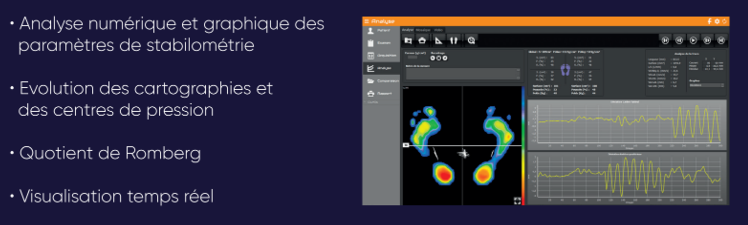
\includegraphics[height=4cm]{images/analyse_marche/WinPod2.png}
        \caption{Outil de visualisation des siganux posturographiques}\label{fig:WinPod2}
    \end{subfigure}
\end{figure}

\subsection{SabotSoft}

SabotSoft est une solution avancée pour les analyses détaillées des oscillations 
corporelles et des déséquilibres posturaux. Il intègre des modèles complexes, 
tels que les vecteurs de vitesse, ou les spectres croisés, souvent utilisés pour 
identifier des pathologies neurologiques spécifiques. Son interface, bien que avancée,
requiert une expertise technique pour être exploitée au maximum. 
Les graphiques et représentations visuelles qu’il propose sont d’une grande précision,
facilitant l’interprétation des données pour des experts en biomécanique ou 
neurologie.

SabotSoft est une solution avancée pour les analyses détaillées 
des oscillations corporelles et des déséquilibres posturaux. 
Cette plateforme d’analyse a comme fonctionnalités : 

\begin{itemize}
    \item \textbf {Statokinésigrammes et ellipses de confiance} 
    \item \textbf {Centre de pressions et centre de masse} 
    \item \textbf {Contrôle et sur-contrôle des oscillations (densité spectrale d’interaction)}
    \item \textbf {Vectogramme du centre de pressions et du centre de masses}
    \begin{itemize}
        \item Distribution des vecteurs vitesse par secteur autour de l’origine.
        \item Détection des singularités et limites du modèle du pendule inversé mono-articulé.
        \item Révélation des blocages fonctionnels (par exemple, non-alignement des axes de cheville) ou des dysfonctions (ex. : jambe courte).
    \end{itemize} 
    \item \textbf{Spectre des forces verticales :}
    \begin{itemize}
    \item Analyse par FFT de la résultante des forces verticales $Z(t)$.
    \item Identification de mouvements verticaux de haute fréquence et de trémors pathologiques.
    \end{itemize}
    \item \textbf{Diagramme des asymétries :}
    \begin{itemize}
    \item Visualisation des asymétries des placements moyens du centre de pressions (CdP).
    \item Comparaison avec une référence normative basée sur une population témoin.
    \item Identification des écarts de position et de direction, illustrés par des vecteurs.
    \item Différences entre les enregistrements en condition yeux ouverts et yeux fermés.
    \end{itemize}
    \item \textbf{Ondelette :}
    \begin{itemize}
        \item Représentation temps-fréquence du signal stabilométrique à l’aide d’ondelettes.
    \item Analyse tridimensionnelle (temps-fréquence-intensité) ou plane (par code couleur).
    \end{itemize}
\end{itemize}



\begin{figure}[H]
    \centering
    \begin{subfigure}[b]{0.45\textwidth}
      \centering
        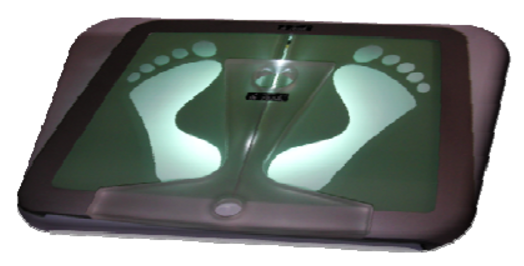
\includegraphics[height=3.5cm]{images/analyse_marche/SabotSoft1.png}
        \caption{Plateforme stabilométriques SobotSoft}\label{fig:sabotsoft1}
    \end{subfigure}
    \begin{subfigure}[b]{0.5\textwidth}
        \centering
        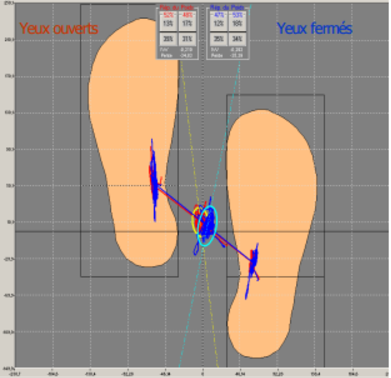
\includegraphics[height=4cm]{images/analyse_marche/SabotSoft2.png}
        \caption{Outil de visualisation de centre de pression yeux ouverts et fermés}\label{fig:SabotSoft23}
    \end{subfigure}\\
    \begin{subfigure}[b]{0.5\textwidth}
        \hspace{-1.5cm} 
        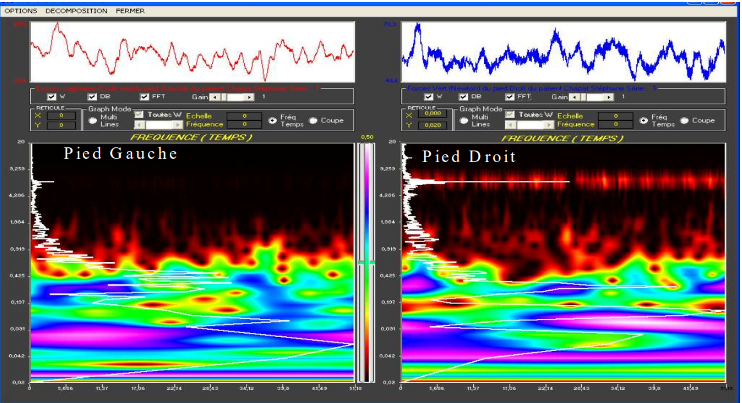
\includegraphics[height=6cm]{images/analyse_marche/SabotSoft5.png}
        \caption{Outil d'analyse de x et y dans le domaine temporel}\label{fig:SabotSoft5}
    \end{subfigure}
\end{figure}


\newpage
\section{Méthodes d'analyse des signaux}

\subsection{Relation entre centre de pression et centre de masse}

Le centre de pression (CdP) reflète les ajustements actifs du corps pour maintenir son équilibre, tandis que le centre de masse (ou centre de gravité, qui sera appelé CdM) est le point théorique correspondant à la position moyenne de la masse corporelle.
Comprendre la relation entre ces deux notions différentes, bien que corrélées, est essentiel pour comprendre comment et par quels mécanismes le corps maintient son équilibre (dans le cas de l'étude, il est question de l'équilibre orthostatique).
Pour maintenir son équilibre, le corps fait osciller son CdP autour du CdM. 
Le corps ajuste constamment la position du CdP afin que les mouvements du CdM (qui sont présents même dans une position debout immobile) ne sorte de la surface du support (la zone délimitée par le contact des deux pieds au sol). 
Si le CdM sort de cette surface, le corps ne peut plus maintenir son équilibre et une chute est alors possible.
Ces ajustements engagés par le corps montrent alors que l'accélération du CdM est proportionnelle à la différence entre le CdM et le CdP; le CdP entraîne le CdM dans la direction opposée à son déplacement afin de maintenir son équilibre.
Une formule de relation entre le CdP et le CdM a été modélisée à partir de l'équation mécanique simple du pendule inversé (représentant cet entraînement opposé du CdP sur le CdM) : 

\[
    CoP = CoM - \frac{h}{g} \times \frac{d^2 CoM}{dt^2}
\]

Les différentes méthodes d'analyse et leurs modèles mathématiques proposés ci-dessous sont applicables au CdM ou au CdP.
La relation mathématique permettant de passer du CdP au CdM décrite plus tôt est utile pour obtenir des résultats plus précis avec les différentes méthodes décrites dans la suite du rapport.
Ce passage de CdP au CdM est facultative et dépend des habitudes et du niveau de précision demandé par les tests cliniques.

\subsection{Analyse spatio-temporelle}

L'analyse spatio-temporelle permet de déterminer la qualité de l'équilibre orthostatique. 
Elle reflète la capacité du corps d'un patient à maintenir un bon équilibre en position stationnaire droite. 
Le signal étudié est la représentation temporelle de la trajectoire du CdM en position statique debout sur une plateforme statique. 
Il est important de rappeler que ces méthodes sont directement applicables avec le CdP.

\subsubsection{Position moyenne du CdM}

La position moyenne du CdM représente la moyenne de l'ensemble des positions successives du CdM. 
Elle est calculée pour deux types de mouvements : les déplacements médio-latéral ($M_{ml}$), ainsi que pour les déplacements antéro-postérieurs ($M_{ap}$).

\[
M_{AP} = \left( \frac{1}{n} \right) \sum_{n=1}^N \mbox{CoM}_{AP}(n)
\]

\[
M_{ML} = \left( \frac{1}{n} \right) \sum_{n=1}^N \mbox{CoM}_{ML}(n)
\]

Où $CoM$ et la pression du centre de masse suivant la direction AP ou la direction ML.

Plus les valeurs sont basses, plus la qualité de l'équilibre est bonne. 
La position moyenne est régulièrement couplée à l'écart-type, afin de pouvoir les situer l'un par rapport à l'autre, et ainsi donner une idée de la dispersion autour de la moyenne.

\subsubsection{Vitesse moyenne du CdM}

La mesure des longueurs des déplacements du centre de masse sur les deux axes (AP et ML) permettent d'estimer l'énergie dépensée pour la régulation de la posture orthostatique.

\[
L_{AP} = \sum_{n=1}^{N-1} \left| \mbox{CoM}_{AP}(n+1) - \mbox{CoM}_{AP}(n) \right| \tag{5}
\]

\[
L_{ML} = \sum_{n=1}^{N-1} \left| \mbox{CoM}_{ML}(n+1) - \mbox{CoM}_{ML}(n) \right| \tag{6}
\]

\[
MV_{AP} = \frac{L_{AP}}{T}
\]
\[
MV_{AP} = \frac{L_{AP}}{T}
\]

Les vitesses ainsi calculées représentent alors le tracé total en fonction du temps. 
Une vitesse élevée signifie un mauvais équilibre. 
Elles peuvent aussi renseigner sur la consommation d'énergie.

\subsubsection{Valeur quadratique moyenne (RMS pour root mean square)}

\[
RMS_{AP} =\sqrt{  \frac{\sum_{n=1}^{N} \left (\text{CoM}_{AP}(n) \right)^2 }{N}}  \tag{9}
\]

\[
RMS_{ML} =\sqrt{  \frac{\sum_{n=1}^{N} \left (\text{CoM}_{ML}(n) \right)^2 }{N}}  \tag{10}
\]

Le calcul des moyennes quadratiques des amplitudes de déplacement du CdM sur les deux axes définis précédemment permet de quantifier l'habileté à maintenir l'équilibre. 
Plus ces mesures sont basses, plus l'habileté est grande.

\subsubsection{Écart maximal}

\[
R_{AP}= max \left ( \text CoM_{AP} \right ) - min\left ( \text CoM_{AP} \right ) \tag{11}
\]


\[R_{ML}= max \left ( \text CoM_{ML} \right ) - min\left ( \text CoM_{ML} \right ) \tag{12}
\]

L'écart maximal est la différence entre la position maximale et minimale du CdM et est défini suivant les deux axes AP et ML. 
Une augmentation d'une de ces valeurs peut être interprétable en une baisse de la capacité à maintenir l'équilibre postural.

\subsubsection{Surface de l'ellipse de confiance (CEA)}

\[
CEA= 6\pi \sqrt{ \left ( \frac{\sum_{n=1}^{N} \left (\text{CoM}_{AP}(n) \right)^2 \times \sum_{n=1}^{N} \left ( \text{CoM}_{ML}(n) \right)^2}{N^2} \right ) - \left (\frac{\sum_{n=1}^N \text{CoM}_{AP} \times CoM_{ML}}{N} \right)^2} \tag{13}
\]

La surface de l'ellipse de confiance regroupe un certain pourcentage du statokinésigramme (en cm2), ici 95\%. 
Cette intervalle de confiance peut varier selon les pratiques ou les habitudes (certains praticiens utilisent une surface d'ellipse de confiance de 90\% par exemple). 
Plus précisément, c'est l'évolution du périmètre de l'ellipse qui est étudiée. 
Plus ce périmètre est grand, et plus l'équilibre est mauvais.

\begin{figure}[ht]
    \centering
    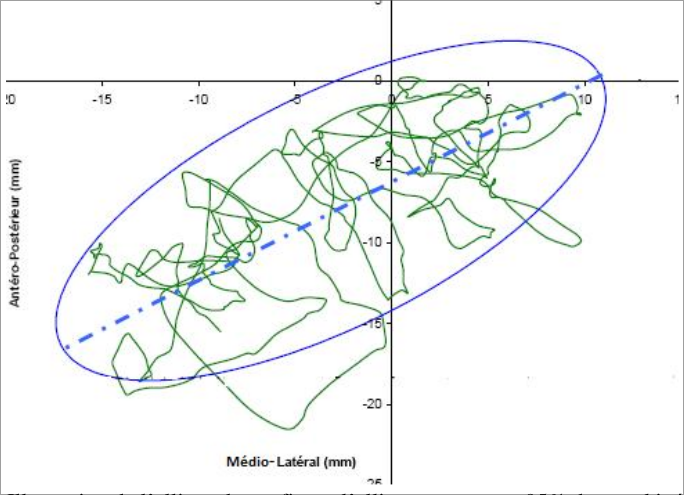
\includegraphics[height=10cm]{images/methode/ellipse_confiance_95.png}
    \caption{Illustration de l'ellipse de confiance (à 95\% du statokinésigramme)}\label{fig:ellipse_confiance}
\end{figure}

\subsubsection{Quotient de Romberg}

\[
QR = \frac{\text{CEA}_{\text{YF}}}{\text{CEA}_{\text{YO}}}\tag{14}
\]

Ce quotient entre la valeur de CEA yeux fermés et la valeur de CEA yeux ouverts permet de mettre en évidence le rôle de la vision dans le contrôle de la posture. 
Une valeur élevée de ce quotient indique une dépendance visuelle accrue dans le maintien de l'équilibre.

\subsection{Analyse spectrale}

L'analyse spectrale se situe dans le domaine fréquentiel. 
Le spectre d'un signal permet d'extraire les différentes composantes présentes dans le signal. 
L'analyse spectrale permet de différencier les différents mécanismes utilisés dans le maintien de l'équilibre en position statique.
Le spectre de fréquence est obtenu en appliquant la transformation de Fourier, principe mathématique, à un signal temporel. 
L'analyse spectrale permet de mettre en évidence l'aspect dynamique du contrôle de la posture orthostatique.

\subsubsection{Fréquence moyenne ou centroïdale}

\[
\text{FM}_{\text{AP}} = \frac{\text{MV}_{\text{AP}}}{4 \cdot \sqrt{2} \cdot \text{M}_{\text{AP}}} \tag{15}
\]

\[
\text{FM}_{\text{ML}} = \frac{\text{MV}_{\text{ML}}}{4 \cdot \sqrt{2} \cdot \text{M}_{\text{ML}}} \tag{16}
\]

La fréquence moyenne est le paramètre qui permet d'étudier le temps nécessaire au mouvement analysé pour revenir dans une position identique. 
Son calcul passe par l'analyse de la distribution fréquentielle des amplitudes.

\subsubsection{Puissance moyenne de la densité spectrale}

La puissance moyenne de la densité spectrale est calculée à partir de l'estimateur de Welch. 
La densité spectrale de puissance permet de mesurer les déplacements du CdP du corps humain.

On part de l'estimation du périodogramme afin de déterminer la densité spectrale de puissance du signal : 

\[
P_{\text{Per}}(f) = \left( \frac{1}{N T_e} \right) \left| \sum_{n=0}^{N-1} x(nT_e)e^{-j2\pi n T_e f} \right|^2
\]

\begin{itemize}
    \item $P_{\text{Per}}(f)$ : C'est le \textbf{périodogramme}, qui est une estimation de la DSP à la fréquence $f$.
    \item $N$ : Nombre d'échantillons du signal.
    \item $T_e$ : Période d'échantillonnage (l'inverse de la fréquence d'échantillonnage, $T_e = \frac{1}{f_e}$, où $f_e$ est la fréquence d'échantillonnage).
    \item $x(nT_e)$ : Valeurs du signal temporel échantillonné à des intervalles $T_e$.
    \item $e^{-j2\pi n T_e f}$ : C'est la base complexe de la transformée de Fourier discrète (TFD) qui décompose le signal en ses composantes fréquentielles.
    \item $\sum_{n=0}^{N-1}$ : La somme sur les échantillons du signal, allant de $n=0$ à $n=N-1$, pour estimer la contribution de chaque fréquence.
    \item $\left| \cdot \right|^2$ : Le carré du module de la transformée de Fourier, qui donne la \textbf{puissance} associée à chaque fréquence.
\end{itemize}

Cette formule est une version discrète du \textbf{périodogramme}, qui permet d'estimer la densité spectrale de puissance d'un signal en fonction de la fréquence $f$. Le processus consiste à :
\begin{itemize}
    \item \textbf{Appliquer la transformée de Fourier discrète (TFD)} au signal $x(nT_e)$ pour transformer le signal temporel en un spectre fréquentiel.
    \item \textbf{Calculer la puissance} à chaque fréquence en prenant le carré du module de la TFD.
    \item \textbf{Normaliser} par $\frac{1}{N T_e}$ pour obtenir une estimation de la DSP, qui représente la distribution de la puissance du signal dans le domaine fréquentiel.
\end{itemize}

Cette estimation permet de voir quelles fréquences contiennent le plus de puissance dans le signal, ce qui est crucial pour l'analyse fréquentielle dans divers domaines, comme la stabilographie, le traitement du signal audio, et d'autres types d'analyse de séries temporelles.

On calcule alors l’estimateur de Welch à partir du périodogramme calculé comme ci-dessus.

\[
P_{Welch}(f) = \frac{1}{L} \sum_{l=1}^{L-1}P_l(f) \tag{18}
\]
\[
P_l(f) = \left( \frac{1}{K}\right) \left |\sum_{n=0}^{K-1} x(n+lK) w(n) e^{-j2\pi nf} \right |^2 \tag{19}
\]

L'estimateur de Welch est une amélioration du périodogramme classique pour estimer la densité spectrale de puissance (DSP) d'un signal. 
Il permet de réduire la variance de l'estimation de la DSP, ce qui en fait une méthode plus robuste pour analyser des signaux bruités ou irréguliers. 
Voici ce que l'estimateur de Welch apporte par rapport au périodogramme simple :

\textbf{1. Réduction de la variance :}
La périodogramme classique a tendance à être un estimateur à variance élevée, c'est-à-dire que ses résultats peuvent fluctuer de manière importante d'un signal à l'autre, même si ceux-ci ont une structure similaire. 
Cela peut rendre l'analyse spectrale moins fiable. 
L'estimateur de Welch réduit cette variance en moyennant plusieurs estimations de la DSP obtenues à partir de segments du signal.

\textbf{2. Segmenter et fenêtrer le signal :}
L'algorithme de Welch divise le signal en plusieurs segments qui se chevauchent partiellement (typiquement de 50\%), et applique une fenêtrage à chaque segment (souvent une fenêtre de Hanning ou de Hamming). 

Ce processus présente plusieurs avantages:
\begin{itemize}
    \item \textbf Segmenter le signal permet de découper le signal en morceaux plus petits, ce qui donne plusieurs petites estimations de la DSP au lieu d'une seule estimation basée sur tout le signal.
    \item \textbf Fenêtrer chaque segment aide à atténuer les discontinuités aux bords des segments, qui pourraient introduire des artefacts dans le domaine fréquentiel, comme des fuites spectrales.
\end{itemize}

\textbf{3. Chevauchement des segments}
Les chevauchements des segments (souvent 50\%) augmentent la quantité d'information utilisée pour chaque estimation locale, améliorant ainsi la stabilité de l'estimation globale. 
Cela permet d'améliorer la résolution fréquentielle tout en conservant une meilleure estimation des puissances.

\textbf{4. Moyenne des DSP :}
Après avoir calculé la transformée de Fourier et le périodogramme pour chaque segment, l'algorithme de Welch prend la moyenne des densités spectrales de puissance (DSP) obtenues. 
Cette moyenne réduit la variance des résultats et améliore la stabilité de l'estimation. 
Le fait de mesurer plusieurs estimations atténue également les fluctuations dues au bruit.

L'estimateur de Welch apporte certains avantages : 
\begin{itemize}
    \item  \textbf{Variance plus fiable} : Comme chaque périodogramme segmenté est moyenné, l'estimateur de Welch a une variance significativement plus fiable que le périodogramme classique, offrant une estimation plus fiable.
    \item \textbf{Meilleure résolution fréquentielle} : Même si chaque segment est plus court que le signal original, l'utilisation du chevauchement permet de conserver une bonne résolution fréquentielle tout en réduisant la variance.
    \item  \textbf{Atténuation des fuites spectrales} : l'application d'une fenêtre sur chaque segment réduit les artefacts induits par les discontinuités aux bords du signal.
\end{itemize}

\begin{figure}[ht]
    \centering
    \begin{subfigure}[b]{0.45\textwidth}
        \centering
        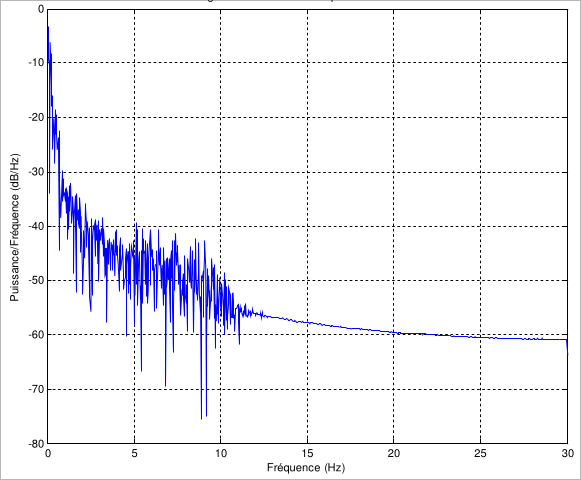
\includegraphics[height=5cm]{images/methode/periodogramme.png}
        \caption{Périodogramme de la densité spectrale de puissance}\label{fig:periodogramme}
    \end{subfigure}
    \begin{subfigure}[b]{0.45\textwidth}
        \centering
        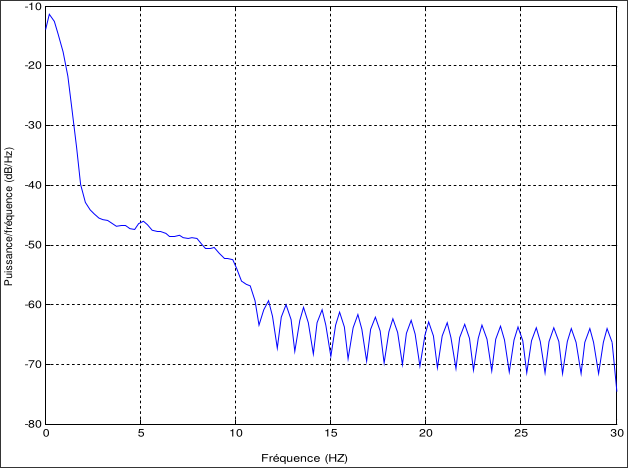
\includegraphics[height=5cm]{images/methode/welch.png}
        \caption{Estimation de Welch de la densité spectrale de puissance}\label{fig:welch}
    \end{subfigure}
    \caption{Comparaison entre le périodogramme et l'estimation de Welch de la densité spectrale de puissance}\label{fig:periodogramme_welch}
\end{figure}


\subsubsection{Pente du spectre de puissance}


Dans le cadre de la stabilographie, l'analyse du spectre dans le 
plan log-log permet de mieux comprendre les mécanismes de régulation
posturale et de quantifier la stabilité ou l'instabilité en 
fonction des fréquences des oscillations du CoP. La régression 
linéaire dans ce contexte permet d'estimer la pente du spectre et 
de révéler les caractéristiques de contrôle postural, avec des 
applications potentielles pour le diagnostic ou la suivi clinique
des troubles de l'équilibre, ou encore pour la prévention des 
chutes chez les personnes âgées.\\


Interprétation en stabilographie : 
\begin{itemize}
\item \textbf Stabilité posturale élevée : 
Lorsque la pente est fortement négative (par exemple au alentour de -2 ou 
plus), cela signifie que la puissance des oscillations posturales 
diminue rapidement avec la fréquence. Dans ce cas, les oscillations 
à basse fréquence dominent, ce qui suggère un contrôle postural 
efficace avec des ajustements lents et stables. Cela pourrait être 
typique chez un jeune adulte en bonne santé.

\item \textbf Instabilité posturale : Lorsque la pente est moins 
négative (par exemple, autour de -1), cela peut signifier que 
les oscillations à haute fréquence contribuent davantage au 
contrôle postural. Ce type de spectre pourrait être observé chez 
des individus plus âgés ou des personnes ayant des troubles de 
l’équilibre, car il indique un contrôle moins stable et une plus 
grande participation des ajustements réflexes ou involontaires.
\end{itemize}


\begin{figure}[H]
    \centering
        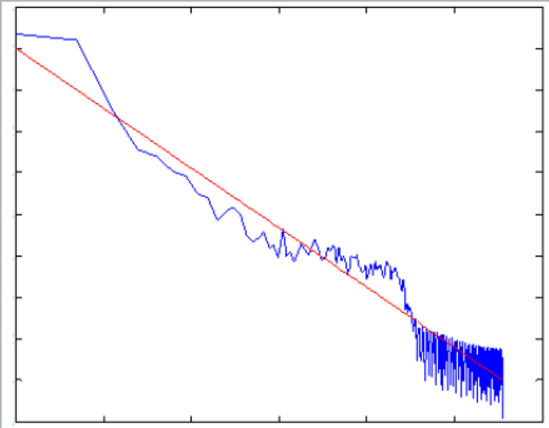
\includegraphics[height=5cm]{images/methode/anaspectrale.png}
        \caption{analyse spectrale et régression linéaire}\label{fig:anaspectrale}
\end{figure}

\end{document}
